\subsubsection{Allgemein}
Im Kapitel \nameref{ch:Content2:sec:Retargeting}
wird eine vorberechnete Textur verwendet. Diese speichert eine
Permutation, die unsere blue noise Textur vom frame t in eine
blue noise Textur vom frame t+1 umwandelt. Diese Permutation wird 
dann auf die Startwerte angewandt bevor das nächste frame t+1 gerendert wird.
Dadurch werden die blue noise Umverteilungen der \nameref{ch:Content2:sec:Sorting} Phase
akkumuliert und die optische Aufwertung erst richtig sichtbar.
Die retarget Textur wird mit Hilfe von \textit{Simulated Annealing} 
\cite{hal02158423} berechnet. Angelehnt an metallurgischen Aufheizen und anschließenden Abkühlen wollen wir eine approximativ 
optimale Lösung finden: Permutiere Pixel der blue noise Textur von 
frame t bis Sie sehr ähnlich verteilt sind wie die Pixel der blue noise
Textur von frame t+1. Dabei ist die Lokalität der Vertauschungen, 
welche wir bereits in der \nameref{ch:Content2:sec:Sorting} Phase
verwendet haben, wichtig. Wir übernehmen hier die Lokalitätsbestimmung aus 
der Arbeit \cite{hal02158423}(Radius r = 6). Von einem hohen Energielevel 
(dither textur zum Zeitpunkt t = 0) wollen wir durch kontrolliertes 
Abkühlen in ein Niederes gelangen(dither textur zum Teitpunkt t = 1).
Zugriff auf die dither Textur berechnet sich für weitere Zeitpunkte
wie hier \ref{alg:Benutzung vorberechneter Texturen} beschrieben.

Die Funktion nach der optimiert wird ist an die Formel aus\cite{georgiev2016blue} angelehnt.
\begin{equation}\label{eq:pixel energy function}
    E(M) = \sum_{p \neq q}E(p,q) = 
           \sum_{p \neq q} \mathrm{e}^{-\frac{\Vert{p_{i}-q_{i}}\Vert^{2}}{\sigma_{i}^{2}} -
           \frac{\Vert{p_{s}-q_{s}}\Vert^{d/2}}{\sigma_{s}^{2}}}
\end{equation}

Wähle nach \cite{ulichney1993void} $\sigma_{i} = 2.1$ und $\sigma_{s} = 1$ 
Zu den Pixeln p,q beschreibt $p_{i}$ und $q_{i}$ ihre jeweiligen Koordinaten.
Und $p_{s}$ und $q_{s}$ sind ihre d-dimensionalen Samplewerte.

Die günstigen Eigenschaften der \nameref{fig:Exponentialfunktion} für das
Schmelzen sind vielfältig \cite{van1987simulated}. Eine ist die Konvergenz 
der Funktion für $\lim\limits_{n \rightarrow -\infty}{\exp{-x}}$.

\begin{figure}[H]
    \centering
    \begin{subfigure}[b]{0.4\textwidth}
        \begin{equation}\label{eq:unsere Energiefunktion}
            P = e^{-(energy(s_{neu}) - energy(s))/ temperature}
        \end{equation}
        \caption{Akzeptanzwahrscheinlichkeitsfunktion}
    \end{subfigure}
    ~ %add desired spacing between images, e. g. ~, \quad, \qquad, \hfill etc. 
      %(or a blank line to force the subfigure onto a new line)
    \begin{subfigure}[b]{0.7\textwidth}
        \centering 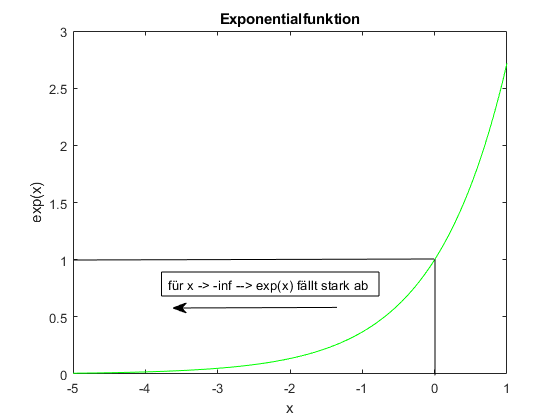
\includegraphics[interpolate=false,width=\linewidth]{content/simulatedAnnealing/Bilder/exponentialfunktion_as_PDF.png}
        \label{fig:Exponentialfunktion}
        \caption{exponentialfunktion}
    \end{subfigure}
    \caption{Die Akzeptanzwahrscheinlichkeitsfunktion P(Energie(s), Energie($s_{new}$), temperature)}
\end{figure}


\begin{algorithm}[H]
    \caption{\textbf{Simulated Annealing} finde eine globale Lösung nahe am Maximum}
    \begin{algorithmic}[1]
        \State initialisiere Startzustand $s=s_{0}$
        \State initialisiere Starttemperatur $T_0$
        \For{i=1...maxSteps}
        \State update Temperatur $t_i$ anhand des Abkühlplanes
        \State //Radius für Nachbarschaftssuche ist auf 6 festgesetzt
        \State $s_{neu}\leftarrow$Nachbarzustand(s)
        \State $energy\Delta = energy(s_{neu}) - energy(s)$
        \If{$energy\Delta < 0$}
        \State s = $s_{new}$
        \Else{}
        \If{P(Energie(s), Energie($s_{new}$), temperature)$\ge$ random(0,1)} 
        \State s = $s_{new}$
        \EndIf
        \EndIf
        \EndFor
        \State return Endzustand s;
    \end{algorithmic}
    \label{alg:retargeting}
\end{algorithm}


Die Wahl der Energiefunktion ist angelehnt an die Formulierung der 
Wahrscheinlichkeitsakzeptanzfunktion in \cite{Kirkpatrick671}. 
Diese wird bedeutet für positive Energydeltas, d.h. wenn der der Energiezustand
des Nachbarn höher als der aktuelle ist. Mit absteigender Temperatur erkennt man 
in der Abbildung \ref{fig:Exponentialfunktion} eine ebenfalls abnehmende Wahrscheinlichkeit
der Akzeptanz. Dies führt zu dem gewünschten Verhalten, energiehöhere Zustände 
zuzulassen, um somit lokale Maxima zu verlassen. Dies geschieht bei höheren 
Temperaturen häufiger wohingegen bei niederen Temperaturen ein gefundenes Maxima
seltener verlassen wird. Höhere Deltas führen passender Weiße zu einem höheren negativen 
Exponenten und damit eine geringere Akzeptanz als Energiezustände, die nur bisschen 
drüber liegen. Die Wahl des Abkühlvorgangs (also das Updaten der Temperatur über die Zeit)
ist problemspezifisch \cite[S. 9]{Kirkpatrick671}. Dabei muss der Abkühlvorgang derart
gewählt werden, sodass kein bloßer Greedy-Algorithmus entsteht und man in einem lokalen 
Maxima stecken bleibt aber auch kein wahlloses Vertauschen entsteht.

Als Startzustand $s_{0}$ definieren wir eine Permutation, die alle 
Elemente auf sich selbst abbildet.
Um von einem Zustand s zu einem neuem Zustand $s_{new}$ zu kommen,
definieren wir eine Nachbarschaftsfunktion \textit{Nachbarzustand()}. 
Diese kann zwei Elemente genau dann vertauschen, wenn Sie in einem 
gegenseitigen Radius r = 6 erreichbar sind. Dabei vertauschen wir
in jedem Schritt ein Pixelpaar. 
Die Wahrscheinlichkeitsfunktion zur neuen Zustandsannahme
P(Energie(s), Energie($s_{new}$)) beschreibt, ob wir den neu
gewählten Zustand $s_{new}$ übernehmen. Dabei wird klassischerweise die
Akzeptanz von Zuständen mit höherer Energie immer kleiner.(bzw. die 
Toleranz gegenüber größeren Fehlern im Bezug zur Zeit). Die allgemeine Akzeptanz von 
Zuständen mit höherer Energie ist dabei von fundamentaler Bedeutung.
Somit verlassen wir möglicherweiße nur lokale Maxima.
Die zu minimierende Energiefunktion \nameref{eq:pixel energy function} betrachtet
dabei zwei 

\subsection{Abkühlfunktion}
Für die Wahl unserer Abkühlfunktion bieten sich einige Optionen.\cite{coolDownOverview}
Im Folgenden wird auf die verschiedenen möglichen Abkühlfunktionen und ihre Eigenschaften
sowie die Wahl interner Parameter(z.B. Starttemperatur) eingegangen. Denn diese Funktion
trägt maßgeblich mit ihrem Konvergenzverhalten zur Effizienz des Abkühlvorgangs bei.
Nach \cite{Kirkpatrick671} wählen wir die Anfangstemperatur $T_0$ derart, dass anfangs jede Neue generierte Lösung akzeptiert(bzw. nahe 1) wird.

\subsubsection{Hajek}

\begin{equation}\label{eq:Hajek}
    f(t) = T_0\log(1+t)
\end{equation}

In \cite{hajek1988cooling} haben wir eine Abkühlfunktion gegeben, welche durch ihre Eigenschaft,
stets gegen das globale Maximum zu konvergieren, unter allen Anderen heraussticht.
Jedoch passiert das asymptotisch extrem langsam. Auch in unseren Fall hat 
es sich als zu langsam herausgestellt.
Leicht aus dem "energetischen" Gleichgewicht zu bringen. Erreicht dann nicht 
das globale Minimum.

\subsubsection{Linear}

\begin{equation}\label{eq:lineare Abkühlung}
    f(t) = T_0 - \mu*t
\end{equation}

Typische Werte für $\alpha$ liegen zwischen 0.8 and 0.99.\cite{Kirkpatrick671}.

\subsubsection{Exponential}
\cite{Kirkpatrick671}

\begin{equation}\label{eq:Exponential}
    f(t) = T_0*pow(alpha,t)
\end{equation}

\subsubsection{Inverse}
\begin{equation}\label{eq:Inverse}
    f(t) = T_0 / (1 + alpha * step)
\end{equation}

\begin{figure}[H]\label{pic:Cool Down Comparisson}
    \centering
    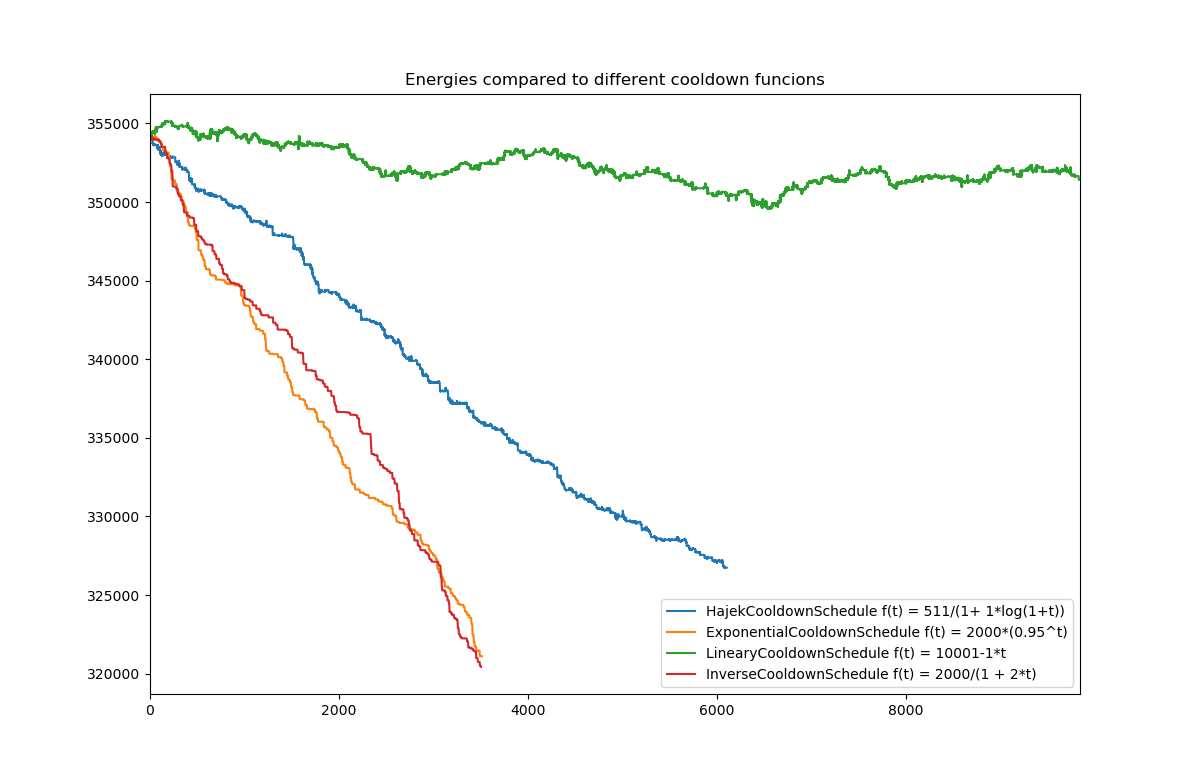
\includegraphics[width=\linewidth]{content/simulatedAnnealing/Bilder/Energy_Cooldown_compared_steps_9842.png}
    \caption{Vergleich von Abkühlfunktionen mit gesetzten Parametern}
\end{figure}

\begin{figure}[H]\label{pic:Retargeting}
    \centering
    \begin{minipage}[t]{0.45\linewidth}
        \centering
        
\includegraphics[interpolate=false,width=\linewidth]{content/simulatedAnnealing/Bilder/LDR_RGBA_64.png}
        \caption{Blue noise Textur 64x64}
    \end{minipage}
    \hfill
    \begin{minipage}[t]{0.45\linewidth}
        \centering
        
\includegraphics[interpolate=false,width=\linewidth]{content/simulatedAnnealing/Bilder/retargeted_texture_10312_swaps.png}
        \caption{Permutation; gespeichert in R,G-Channel einer .png}
    \end{minipage}
\end{figure}

\subsubsection{Energieverlauf}

\begin{figure}[H]\label{pic:Energy Annealing}
    \centering
    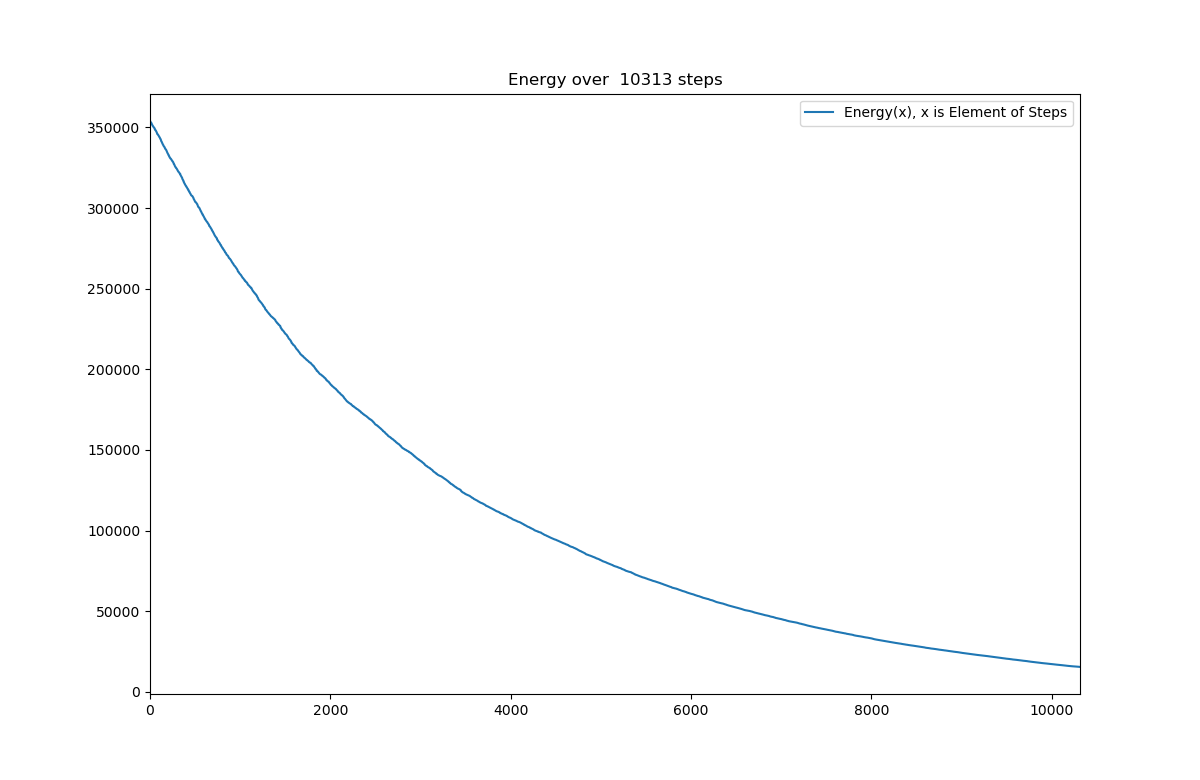
\includegraphics[width=\linewidth]{content/simulatedAnnealing/Bilder/Energy_10313_steps.png}
    \caption{Energieverlauf beim Simulated Annealing}
\end{figure}

\begin{figure}[H]\label{pic:Akzeptanzfunktionsverlauf}
    \centering
    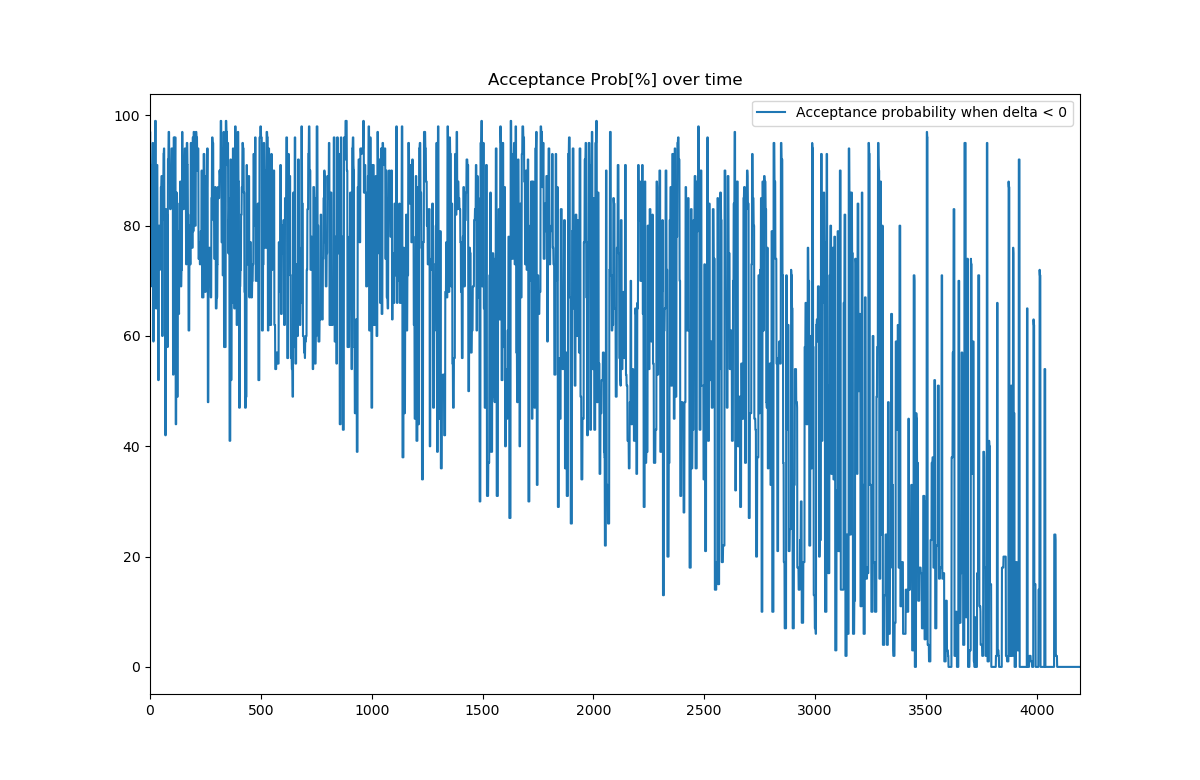
\includegraphics[width=\linewidth]{content/simulatedAnnealing/Bilder/Acceptance_Probabilities over time 4195_steps_LinearyCooldownSchedule.png}
    \caption{Akzeptanzfunktionsverlauf bei negativen Energiedeltas}
\end{figure}






